\documentclass[twoside]{article}\usepackage[]{graphicx}\usepackage[]{color}
% maxwidth is the original width if it is less than linewidth
% otherwise use linewidth (to make sure the graphics do not exceed the margin)
\makeatletter
\def\maxwidth{ %
  \ifdim\Gin@nat@width>\linewidth
    \linewidth
  \else
    \Gin@nat@width
  \fi
}
\makeatother

\definecolor{fgcolor}{rgb}{0.345, 0.345, 0.345}
\newcommand{\hlnum}[1]{\textcolor[rgb]{0.686,0.059,0.569}{#1}}%
\newcommand{\hlstr}[1]{\textcolor[rgb]{0.192,0.494,0.8}{#1}}%
\newcommand{\hlcom}[1]{\textcolor[rgb]{0.678,0.584,0.686}{\textit{#1}}}%
\newcommand{\hlopt}[1]{\textcolor[rgb]{0,0,0}{#1}}%
\newcommand{\hlstd}[1]{\textcolor[rgb]{0.345,0.345,0.345}{#1}}%
\newcommand{\hlkwa}[1]{\textcolor[rgb]{0.161,0.373,0.58}{\textbf{#1}}}%
\newcommand{\hlkwb}[1]{\textcolor[rgb]{0.69,0.353,0.396}{#1}}%
\newcommand{\hlkwc}[1]{\textcolor[rgb]{0.333,0.667,0.333}{#1}}%
\newcommand{\hlkwd}[1]{\textcolor[rgb]{0.737,0.353,0.396}{\textbf{#1}}}%
\let\hlipl\hlkwb

\usepackage{framed}
\makeatletter
\newenvironment{kframe}{%
 \def\at@end@of@kframe{}%
 \ifinner\ifhmode%
  \def\at@end@of@kframe{\end{minipage}}%
  \begin{minipage}{\columnwidth}%
 \fi\fi%
 \def\FrameCommand##1{\hskip\@totalleftmargin \hskip-\fboxsep
 \colorbox{shadecolor}{##1}\hskip-\fboxsep
     % There is no \\@totalrightmargin, so:
     \hskip-\linewidth \hskip-\@totalleftmargin \hskip\columnwidth}%
 \MakeFramed {\advance\hsize-\width
   \@totalleftmargin\z@ \linewidth\hsize
   \@setminipage}}%
 {\par\unskip\endMakeFramed%
 \at@end@of@kframe}
\makeatother

\definecolor{shadecolor}{rgb}{.97, .97, .97}
\definecolor{messagecolor}{rgb}{0, 0, 0}
\definecolor{warningcolor}{rgb}{1, 0, 1}
\definecolor{errorcolor}{rgb}{1, 0, 0}
\newenvironment{knitrout}{}{} % an empty environment to be redefined in TeX

\usepackage{alltt}
\usepackage[utf8]{inputenc}
\usepackage[czech]{babel}
\usepackage{fancyhdr}
\usepackage[paper=a4paper, nomarginpar, foot=1.5cm, top=2.5cm, bottom=2.5cm, left=2.5cm, right=2.5cm]{geometry}
\usepackage{siunitx}

\pagestyle{fancy}
\fancyhead{} % clear all header fields
\fancyhead[RO,LE]{Marek Földi}
\fancyhead[RE,LO]{Úkol 1}
\fancyfoot{} % clear all footer fields
\fancyfoot[LE,RO]{\thepage}

\addto\captionsczech{\renewcommand{\figurename}{Graf. č.}}
\IfFileExists{upquote.sty}{\usepackage{upquote}}{}
\begin{document}





\subsection*{Příklad 1:}
\begin{knitrout}
\definecolor{shadecolor}{rgb}{0.969, 0.969, 0.969}\color{fgcolor}\begin{kframe}
\begin{alltt}
\hlkwd{mean}\hlstd{(zapesti.leve)}
\end{alltt}
\begin{verbatim}
## [1] 157.7857
\end{verbatim}
\begin{alltt}
\hlkwd{median}\hlstd{(zapesti.leve)}
\end{alltt}
\begin{verbatim}
## [1] 155
\end{verbatim}
\begin{alltt}
\hlkwd{quantile}\hlstd{(zapesti.leve)}
\end{alltt}
\begin{verbatim}
##   0%  25%  50%  75% 100% 
##  130  150  155  165  201
\end{verbatim}
\begin{alltt}
\hlkwd{sd}\hlstd{(zapesti.leve)}
\end{alltt}
\begin{verbatim}
## [1] 12.38634
\end{verbatim}
\begin{alltt}
\hlkwd{mean}\hlstd{(bota)}
\end{alltt}
\begin{verbatim}
## [1] 40.04643
\end{verbatim}
\begin{alltt}
\hlkwd{median}\hlstd{(bota)}
\end{alltt}
\begin{verbatim}
## [1] 39
\end{verbatim}
\begin{alltt}
\hlkwd{quantile}\hlstd{(bota)}
\end{alltt}
\begin{verbatim}
##   0%  25%  50%  75% 100% 
##   36   38   39   42   48
\end{verbatim}
\begin{alltt}
\hlkwd{sd}\hlstd{(bota)}
\end{alltt}
\begin{verbatim}
## [1] 2.71281
\end{verbatim}
\end{kframe}
\end{knitrout}

Průměr šířky levého zápěstí je 157,79~\si{\milli\metre}, medián je 155~\si{\milli\metre}, první kvartily 150~\si{\milli\metre}, třetí kvartil 165~\si{\milli\metre} a směrodatná odchylka je 12,39. Průměr velikosti bot je 40,05, medián je 39, první kvartil 38, třetí kvartil 42 a směrodatná odchylka je 2,71.

\subsection*{Příklad 2:}
\begin{knitrout}
\definecolor{shadecolor}{rgb}{0.969, 0.969, 0.969}\color{fgcolor}\begin{kframe}
\begin{alltt}
\hlkwd{cor}\hlstd{(zapesti.leve, bota)}
\end{alltt}
\begin{verbatim}
## [1] 0.6784696
\end{verbatim}
\end{kframe}
\end{knitrout}

Z~korelačního koeficientu můžeme říct, že hodnoty na sobě pozitivně závisí. Závislost můžeme také pozorovat na \emph{scatterplot}, viz. grafu č. \ref{fig:plot2}.
\begin{knitrout}
\definecolor{shadecolor}{rgb}{0.969, 0.969, 0.969}\color{fgcolor}\begin{kframe}
\begin{alltt}
\hlkwd{scatterplot}\hlstd{(zapesti.leve}\hlopt{~}\hlstd{bota,} \hlkwc{regLine}\hlstd{=}\hlnum{TRUE}\hlstd{,} \hlkwc{smooth}\hlstd{=}\hlnum{FALSE}\hlstd{,} \hlkwc{boxplots}\hlstd{=}\hlnum{FALSE}\hlstd{,}
    \hlkwc{xlab}\hlstd{=}\hlstr{"Velikost boty"}\hlstd{,} \hlkwc{ylab}\hlstd{=}\hlstr{"Šířka levého zápěstí v mm"}\hlstd{)}
\end{alltt}
\end{kframe}\begin{figure}[h]
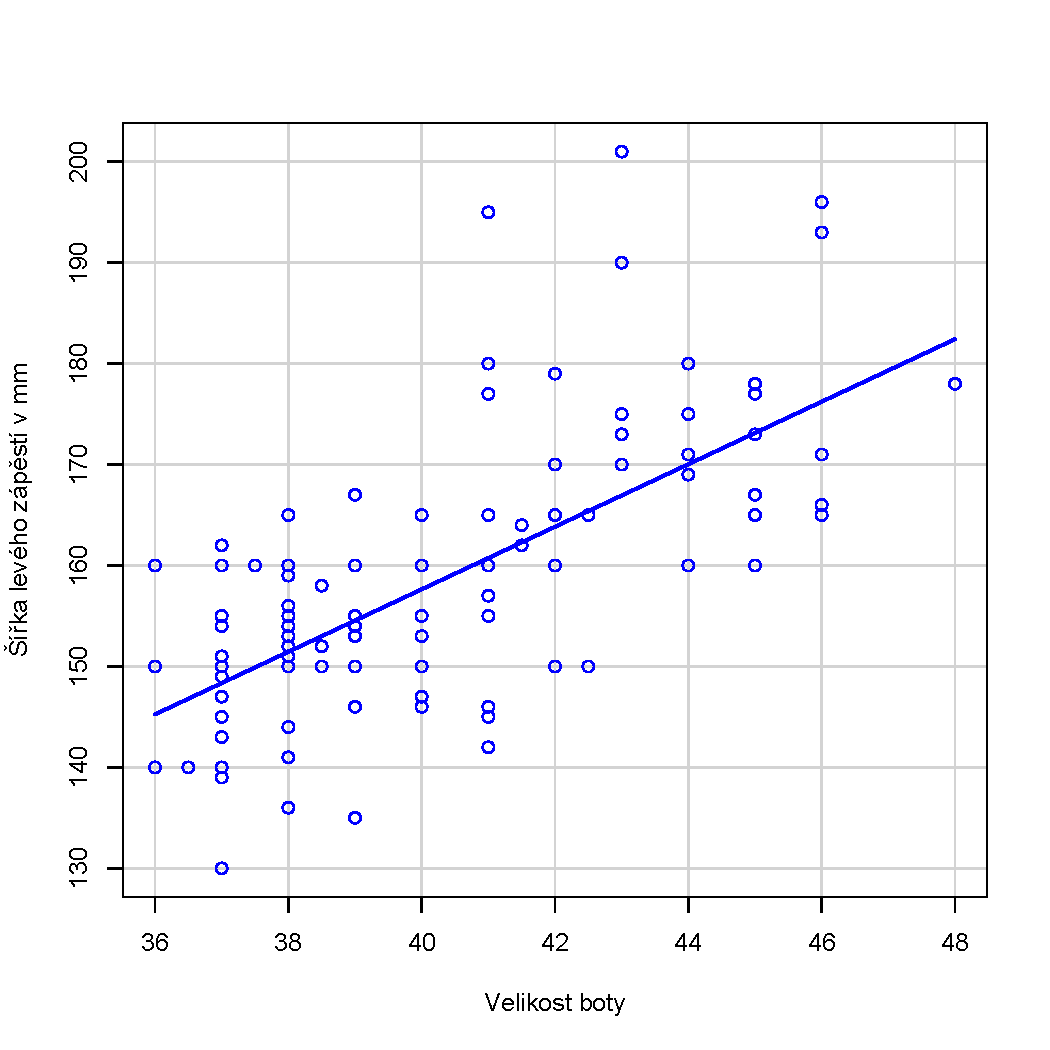
\includegraphics[width=\maxwidth]{figure/plot2-1} \caption[Závislost mezi velikostí bot a velikosti zápěstí]{Závislost mezi velikostí bot a velikosti zápěstí}\label{fig:plot2}
\end{figure}


\end{knitrout}


\newpage
\subsection*{Příklad 3:}
\begin{knitrout}
\definecolor{shadecolor}{rgb}{0.969, 0.969, 0.969}\color{fgcolor}\begin{kframe}
\begin{alltt}
\hlkwd{numSummary}\hlstd{(zapesti.leve,} \hlkwc{groups}\hlstd{=pohlavi,} \hlkwc{statistics}\hlstd{=}\hlkwd{c}\hlstd{(}\hlstr{"mean"}\hlstd{,} \hlstr{"sd"}\hlstd{,} \hlstr{"quantiles"}\hlstd{),}
    \hlkwc{quantiles}\hlstd{=}\hlkwd{c}\hlstd{(}\hlnum{0}\hlstd{,}\hlnum{.25}\hlstd{,}\hlnum{.5}\hlstd{,}\hlnum{.75}\hlstd{,}\hlnum{1}\hlstd{))}
\end{alltt}
\begin{verbatim}
##       mean        sd  0% 25% 50% 75% 100% data:n
## F 152.9126  8.212982 130 150 153 160  179    103
## M 171.3514 12.007443 150 165 170 177  201     37
\end{verbatim}
\end{kframe}
\end{knitrout}
V~testovaném souboru je 103 žen a 37 mužů. Průměry velikosti zápěstí se mezi pohlavím liší. U~mužů je větší než u~žen. Rozdíl průměrů můžeme sledovat i na \emph{plot of means}, viz. graf č. \ref{fig:plot3}.

\begin{knitrout}
\definecolor{shadecolor}{rgb}{0.969, 0.969, 0.969}\color{fgcolor}\begin{kframe}
\begin{alltt}
\hlkwd{plotMeans}\hlstd{(zapesti.leve, pohlavi,} \hlkwc{error.bars}\hlstd{=}\hlstr{"se"}\hlstd{,} \hlkwc{main}\hlstd{=}\hlstr{""}\hlstd{,} \hlkwc{connect}\hlstd{=}\hlnum{FALSE}\hlstd{,}
    \hlkwc{xlab}\hlstd{=}\hlstr{"Pohlaví"}\hlstd{,} \hlkwc{ylab}\hlstd{=}\hlstr{"Průměr šířky levého zápěstí v mm"}\hlstd{)}
\end{alltt}
\end{kframe}\begin{figure}[h]
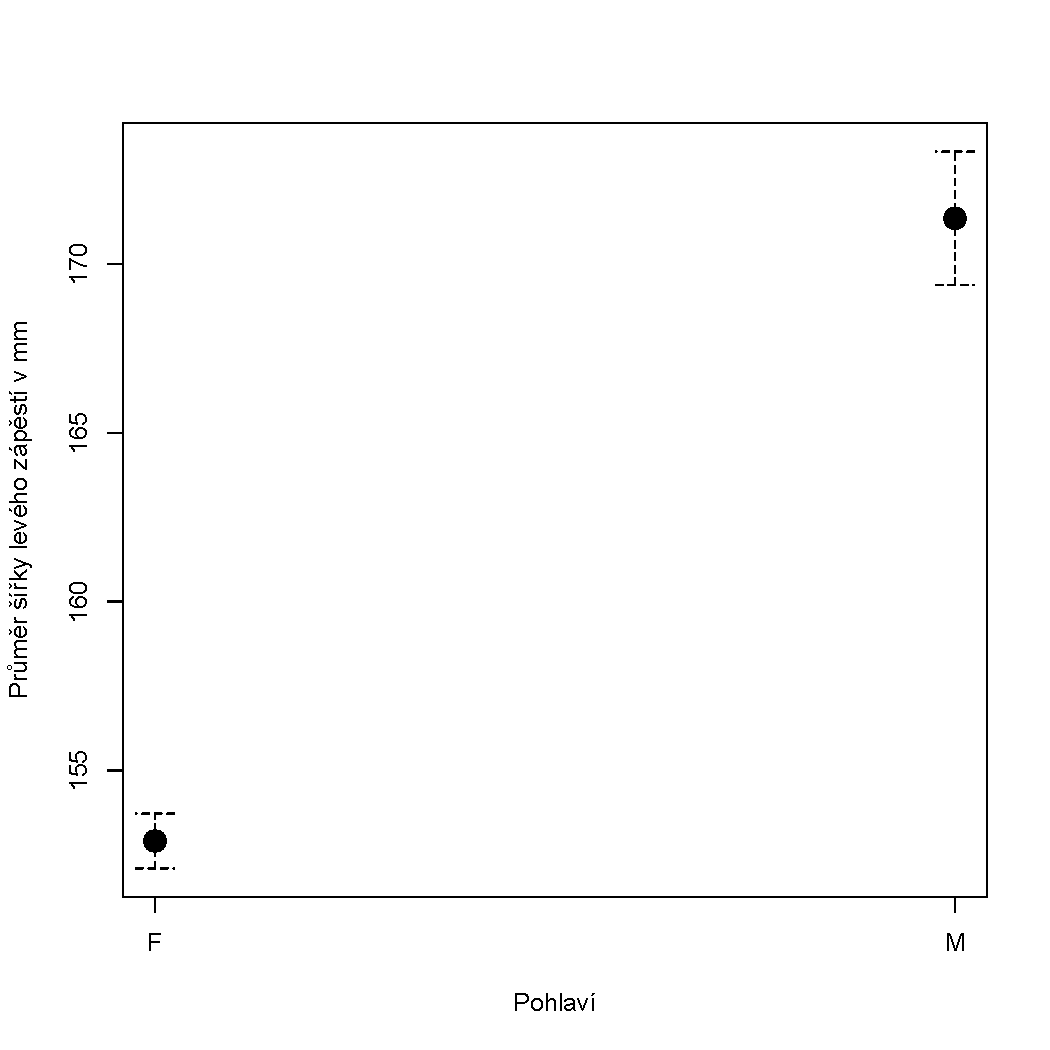
\includegraphics[width=\maxwidth]{figure/plot3-1} \caption[Závislost mezi pohlavím a velikosti zápěstí]{Závislost mezi pohlavím a velikosti zápěstí}\label{fig:plot3}
\end{figure}


\end{knitrout}

\newpage
\subsection*{Příklad 4:}
\begin{knitrout}
\definecolor{shadecolor}{rgb}{0.969, 0.969, 0.969}\color{fgcolor}\begin{kframe}
\begin{alltt}
\hlkwd{cor}\hlstd{(zapesti.leve[pohlavi} \hlopt{==} \hlstr{"F"}\hlstd{], bota[pohlavi} \hlopt{==} \hlstr{"F"}\hlstd{])}
\end{alltt}
\begin{verbatim}
## [1] 0.4011325
\end{verbatim}
\begin{alltt}
\hlkwd{cor}\hlstd{(zapesti.leve[pohlavi} \hlopt{==} \hlstr{"M"}\hlstd{], bota[pohlavi} \hlopt{==} \hlstr{"M"}\hlstd{])}
\end{alltt}
\begin{verbatim}
## [1] 0.2453717
\end{verbatim}
\end{kframe}
\end{knitrout}
U~žen je korelace vyšší a to 0,40. U~mužů je korelace menší a to 0,25. U~obou pohlaví je závislost kladná. Rozdíly v~korelaci můžeme pozorovat i na \emph{scatterplot}, viz. graf č. \ref{fig:plot4}

\begin{knitrout}
\definecolor{shadecolor}{rgb}{0.969, 0.969, 0.969}\color{fgcolor}\begin{kframe}
\begin{alltt}
\hlkwd{scatterplot}\hlstd{(zapesti.leve}\hlopt{~}\hlstd{bota} \hlopt{|} \hlstd{pohlavi,} \hlkwc{regLine}\hlstd{=}\hlnum{TRUE}\hlstd{,} \hlkwc{smooth}\hlstd{=}\hlnum{FALSE}\hlstd{,}
    \hlkwc{boxplots}\hlstd{=}\hlnum{FALSE}\hlstd{,} \hlkwc{by.groups}\hlstd{=}\hlnum{TRUE}\hlstd{,} \hlkwc{xlab}\hlstd{=}\hlstr{"Velikost bot"}\hlstd{,}
    \hlkwc{ylab}\hlstd{=}\hlstr{"Šířka levého zápěstí v mm"}\hlstd{)}
\end{alltt}
\end{kframe}\begin{figure}[h]
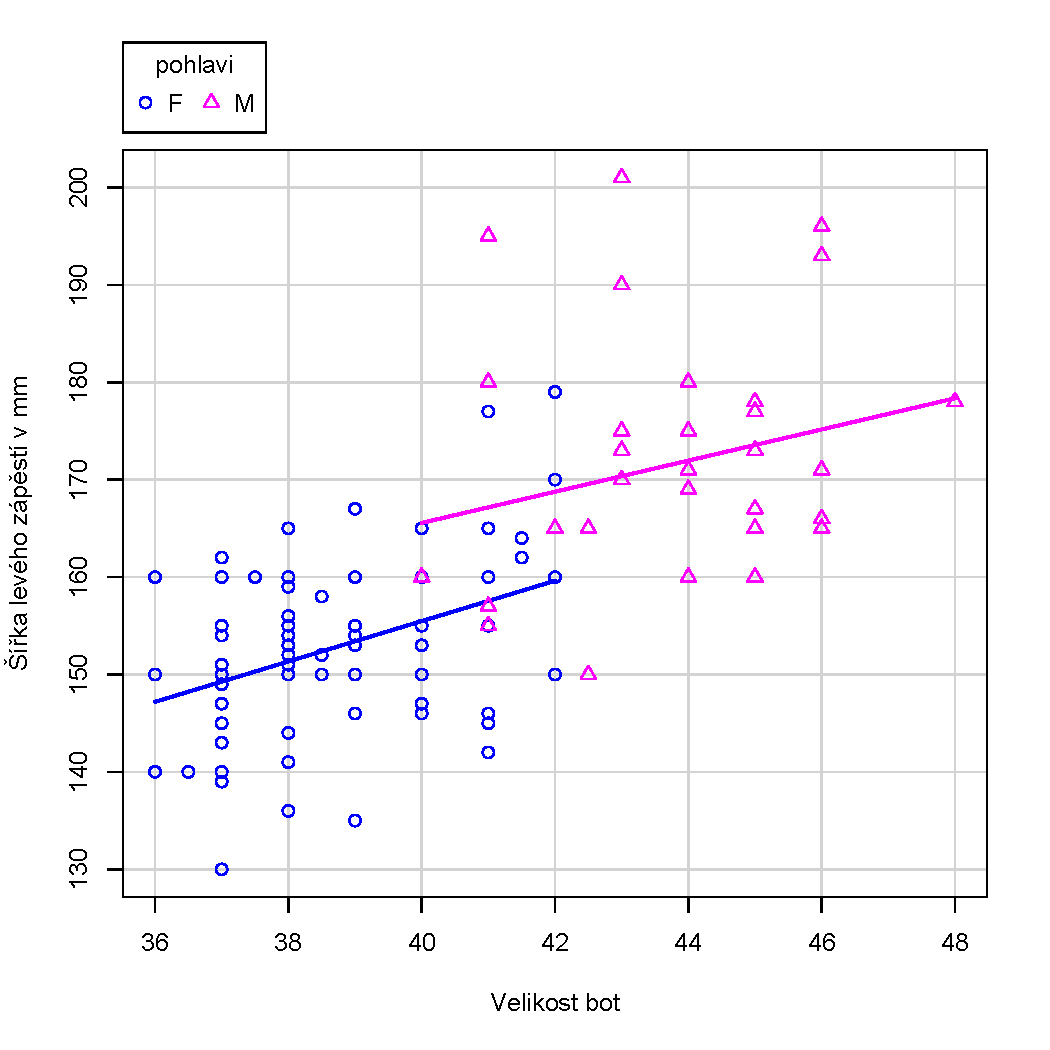
\includegraphics[width=\maxwidth]{figure/plot4-1} \caption[Závislost mezi velikostí bot a velikosti zápěstí pro pohlaví odděleně]{Závislost mezi velikostí bot a velikosti zápěstí pro pohlaví odděleně}\label{fig:plot4}
\end{figure}


\end{knitrout}

\subsection*{Příklad 5:}
\begin{knitrout}
\definecolor{shadecolor}{rgb}{0.969, 0.969, 0.969}\color{fgcolor}\begin{kframe}
\begin{alltt}
\hlstd{fsport} \hlkwb{<-} \hlkwd{Recode}\hlstd{(sport,} \hlstr{'0="0"; 1:2="1-2"; 2.5:5="2,5-5"; 5.5:15="5,5-15"'}\hlstd{,}
    \hlkwc{as.factor}\hlstd{=}\hlnum{TRUE}\hlstd{)}
\hlkwd{summary}\hlstd{(fsport)}
\end{alltt}
\begin{verbatim}
##      0    1-2  2,5-5 5,5-15   NA's 
##     19     39     57     24      1
\end{verbatim}
\end{kframe}
\end{knitrout}

Sportu se nevěnuje 19 studentů, hodinu až dvě sportu věnuje 39 studentů, 57 studentů věnuje sportu mezi dvěma a půl hodinou až pěti hodinami, 24 student věnuje sportu mezi pět a půl až patnácti hodinami. Rozdělení studentů mžeme pozorovat na \emph{barplot}, viz. graf. č. \ref{fig:plot5}.

\begin{knitrout}
\definecolor{shadecolor}{rgb}{0.969, 0.969, 0.969}\color{fgcolor}\begin{kframe}
\begin{alltt}
\hlkwd{Barplot}\hlstd{(fsport,} \hlkwc{xlab}\hlstd{=}\hlstr{"Počet hodin sportovních aktivit týdně"}\hlstd{,} \hlkwc{ylab}\hlstd{=}\hlstr{"Počet studentů"}\hlstd{,}
    \hlkwc{label.bars}\hlstd{=}\hlnum{TRUE}\hlstd{)}
\end{alltt}
\end{kframe}\begin{figure}[h]
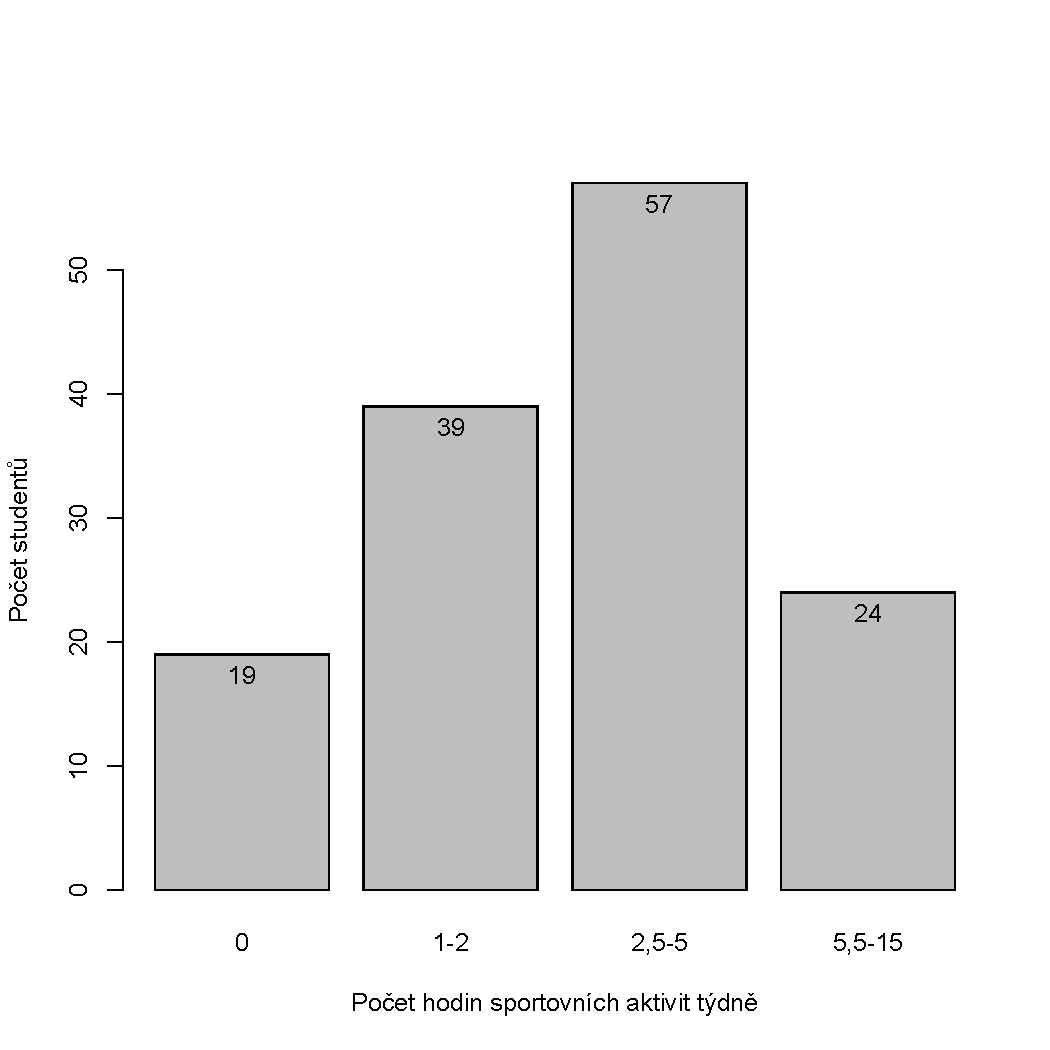
\includegraphics[width=\maxwidth]{figure/plot5-1} \caption[Rozdělní studentů podle počtu hodin sportovních aktivit týdně]{Rozdělní studentů podle počtu hodin sportovních aktivit týdně}\label{fig:plot5}
\end{figure}


\end{knitrout}

\newpage
\subsection*{Příklad 6:}
\begin{knitrout}
\definecolor{shadecolor}{rgb}{0.969, 0.969, 0.969}\color{fgcolor}\begin{kframe}
\begin{alltt}
\hlkwd{numSummary}\hlstd{(tep,} \hlkwc{groups}\hlstd{=fsport,} \hlkwc{statistics}\hlstd{=}\hlkwd{c}\hlstd{(}\hlstr{"mean"}\hlstd{,} \hlstr{"sd"}\hlstd{,} \hlstr{"quantiles"}\hlstd{),}
    \hlkwc{quantiles}\hlstd{=}\hlkwd{c}\hlstd{(}\hlnum{0}\hlstd{,}\hlnum{.25}\hlstd{,}\hlnum{.5}\hlstd{,}\hlnum{.75}\hlstd{,}\hlnum{1}\hlstd{))}
\end{alltt}
\begin{verbatim}
##            mean       sd 0%   25% 50%   75%  100% data:n data:NA
## 0      79.61111 13.35550 60 71.25  77 88.50 108.0     18       1
## 1-2    78.83333 11.75536 50 72.00  78 84.00 104.5     39       0
## 2,5-5  74.41071 11.97995 50 66.00  75 81.25 109.0     56       1
## 5,5-15 73.29167 12.24915 56 62.00  72 84.00  98.0     24       0
\end{verbatim}
\end{kframe}
\end{knitrout}

Průměr tepové frekvenci v~klidu po 1 minutu klesá s~rostoucím počtem hodin věnovaných sportu. Rozdíly v~průměrech jsou pozorovatelné na \emph{plot of means}, viz. graf. č. \ref{fig:plot6}.

\begin{knitrout}
\definecolor{shadecolor}{rgb}{0.969, 0.969, 0.969}\color{fgcolor}\begin{kframe}
\begin{alltt}
\hlkwd{plotMeans}\hlstd{(tep, fsport,} \hlkwc{error.bars}\hlstd{=}\hlstr{"se"}\hlstd{,} \hlkwc{main}\hlstd{=}\hlstr{""}\hlstd{,} \hlkwc{connect}\hlstd{=}\hlnum{FALSE}\hlstd{,}
    \hlkwc{xlab}\hlstd{=}\hlstr{"Počet hodin sportovních aktivit týdně"}\hlstd{,}
    \hlkwc{ylab}\hlstd{=}\hlstr{"Průměr tepové frekvence v klidu po 1 min"}\hlstd{)}
\end{alltt}
\end{kframe}\begin{figure}[h]
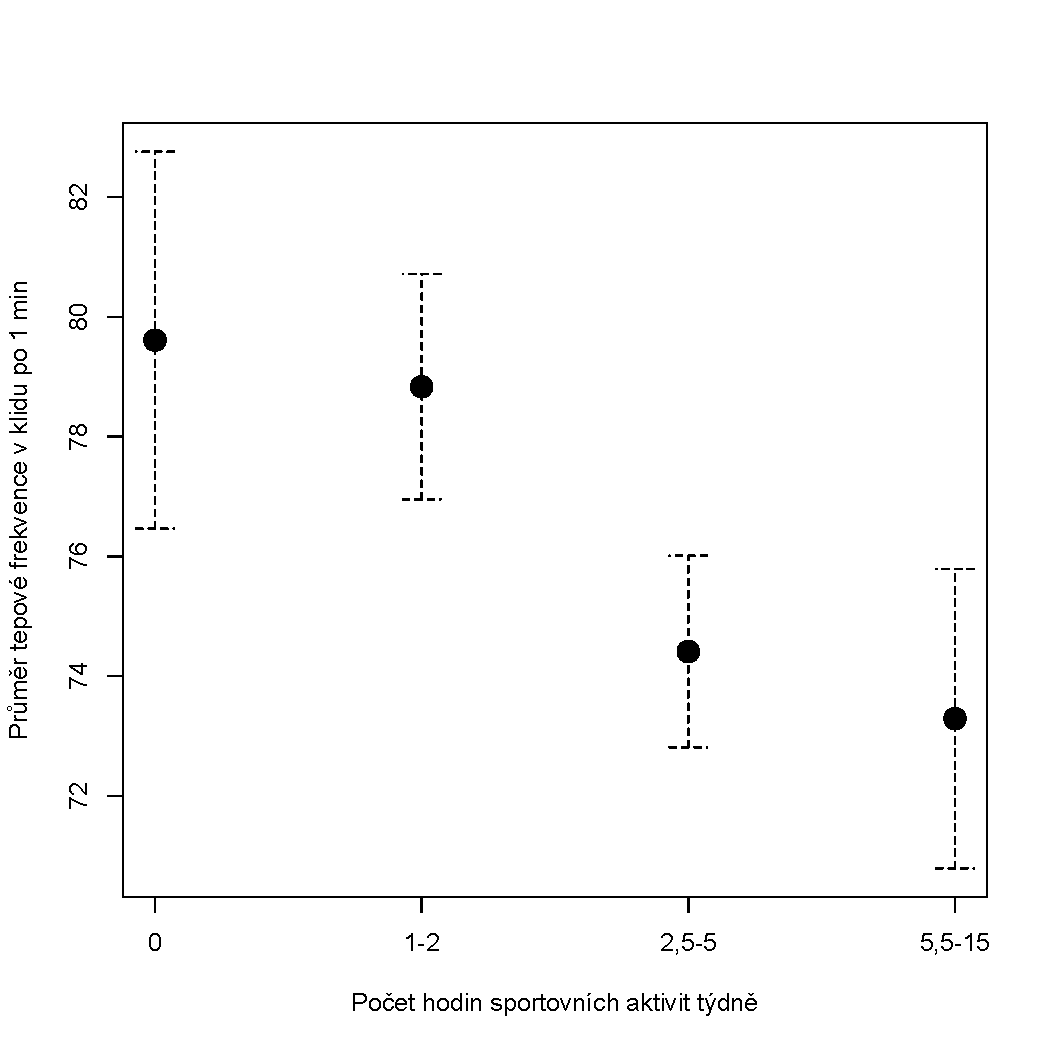
\includegraphics[width=\maxwidth]{figure/plot6-1} \caption[Závislost tepové frekvence a počtu hodin sportovních aktivit týdně]{Závislost tepové frekvence a počtu hodin sportovních aktivit týdně}\label{fig:plot6}
\end{figure}


\end{knitrout}

\subsection*{Příklad 7:}
\begin{knitrout}
\definecolor{shadecolor}{rgb}{0.969, 0.969, 0.969}\color{fgcolor}\begin{kframe}
\begin{alltt}
\hlkwd{table}\hlstd{(hudba,fsport)}
\end{alltt}
\begin{verbatim}
##      fsport
## hudba  0 1-2 2,5-5 5,5-15
##     A 11  27    23     10
##     N  8  12    34     14
\end{verbatim}
\end{kframe}
\end{knitrout}

Hře na hudební nástroj se více věnují studenti, kteří věnují sportu pod dvě hodiny, avšak studenti, kteří se nevěnují sportu vůbec hrají na hudební nástroje méně než studenti, kteří sportu věnují hodinu až dvě. U~studentů, kteří se sportu věnují nad dvě a půl hodiny je zastoupení studentů hrajících na hudební nástroj podobný. Zastoupení studentů hrající na hudební nástroj a studentů nehrající můžeme pozorovat na grafu č. \ref{fig:plot7}.

\begin{knitrout}
\definecolor{shadecolor}{rgb}{0.969, 0.969, 0.969}\color{fgcolor}\begin{kframe}
\begin{alltt}
\hlkwd{plot}\hlstd{(hudba}\hlopt{~}\hlstd{fsport,} \hlkwc{xlab}\hlstd{=}\hlstr{"Počet hodin sportovních aktivit týdně"}\hlstd{,}
    \hlkwc{ylab}\hlstd{=}\hlstr{"Hraje na hudební nástroj"}\hlstd{)}
\end{alltt}
\end{kframe}\begin{figure}[h]
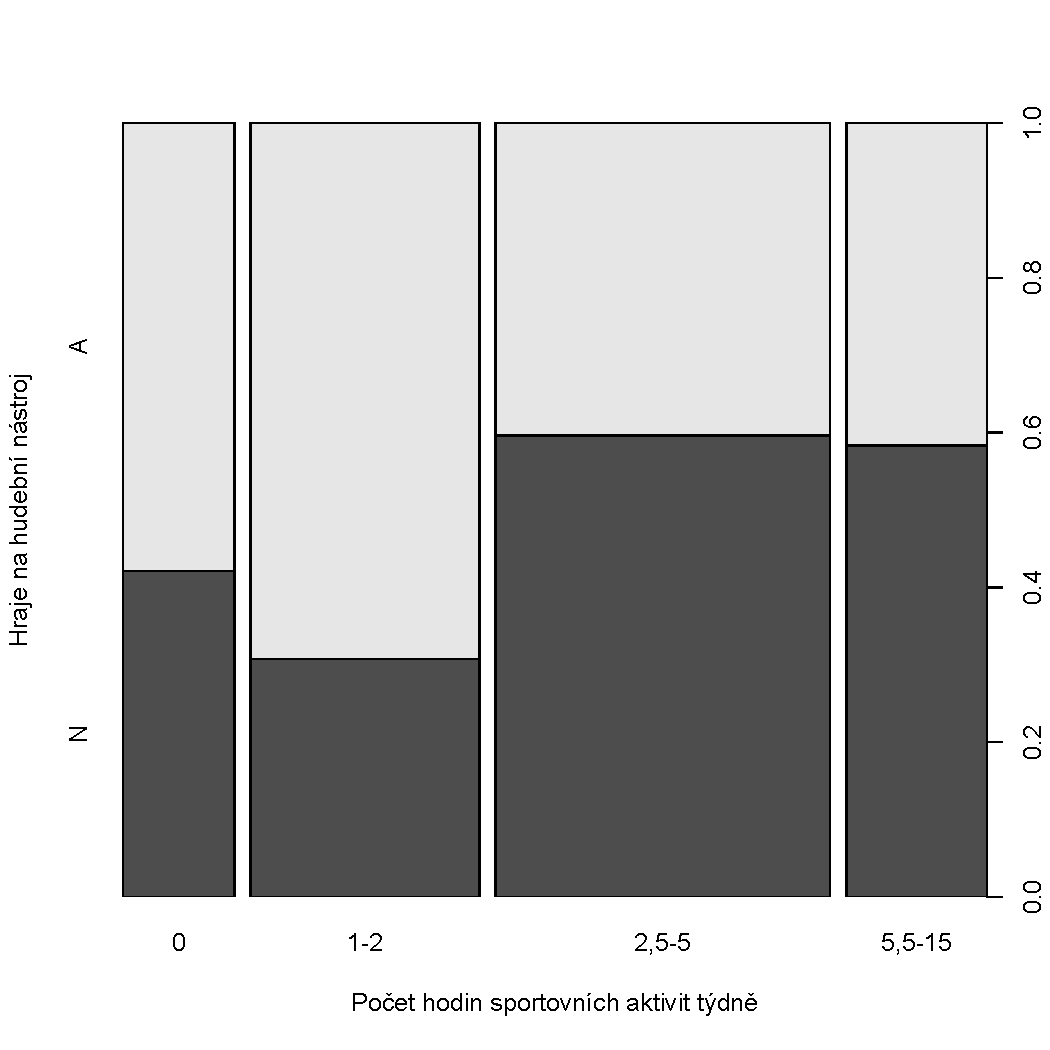
\includegraphics[width=\maxwidth]{figure/plot7-1} \caption[Závislost počtu hodin sportovních aktivit a hraním na hudební nástroj]{Závislost počtu hodin sportovních aktivit a hraním na hudební nástroj}\label{fig:plot7}
\end{figure}


\end{knitrout}

\end{document}
